% Copyright 2004 by Till Tantau <tantau@users.sourceforge.net>.
%
% In principle, this file can be redistributed and/or modified under
% the terms of the GNU Public License, version 2.
%
% However, this file is supposed to be a template to be modified
% for your own needs. For this reason, if you use this file as a
% template and not specifically distribute it as part of a another
% package/program, I grant the extra permission to freely copy and
% modify this file as you see fit and even to delete this copyright
% notice. 

\documentclass{beamer}

% There are many different themes available for Beamer. A comprehensive
% list with examples is given here:
% http://deic.uab.es/~iblanes/beamer_gallery/index_by_theme.html
% You can uncomment the themes below if you would like to use a different
% one:
%\usetheme{AnnArbor}
%\usetheme{Antibes}
%\usetheme{Bergen}
%\usetheme{Berkeley}
%\usetheme{Berlin}
%\usetheme{Boadilla}
%\usetheme{boxes}
%\usetheme{CambridgeUS}
%\usetheme{Copenhagen}
%\usetheme{Darmstadt}
%\usetheme{default}
%\usetheme{Frankfurt}
%\usetheme{Goettingen}
%\usetheme{Hannover}
%\usetheme{Ilmenau}
%\usetheme{JuanLesPins}
%\usetheme{Luebeck}
\usetheme{Madrid}
%\usetheme{Malmoe}
%\usetheme{Marburg}
%\usetheme{Montpellier}
%\usetheme{PaloAlto}
%\usetheme{Pittsburgh}
%\usetheme{Rochester}
%\usetheme{Singapore}
%\usetheme{Szeged}
%\usetheme{Warsaw}


% Customize Warsaw color 
\setbeamercolor*{palette primary}{use=structure,fg=white,bg=red!50!black}
\setbeamercolor*{palette secondary}{use=structure,fg=white,bg=red!60!black}
\setbeamercolor*{palette tertiary}{use=structure,fg=white,bg=red!70!black}

% Customize Warsaw block title and background colors
\setbeamercolor{block title}{bg=red!50!black,fg=white}


% List your packages here

\usepackage[colorinlistoftodos]{todonotes}


\title[Progress Update]{A Generalized Open Source Platform for Building Energy Management}

% % A subtitle is optional and this may be deleted
% \subtitle{Product Proposal}

\author[B.~Lauer]{Brian~Lauer\\\and
Advisor: Dr. Suruz Miah}
% - Give the names in the same order as the appear in the paper.
% - Use the \inst{?} command only if the authors have different
%   affiliation.

\institute[Bradley University] % (optional, but mostly needed)
{
  Department of Electrical and Computer Engineering\\
  Bradley University\\
  1501 W. Bradley Avenue\\
  Peoria, IL, 61625, USA
}
% - Use the \inst command only if there are several affiliations.
% - Keep it simple, no one is interested in your street address.

\date[May~29,~2020]{Friday, May~29,~2020}
% - Either use conference name or its abbreviation.
% - Not really informative to the audience, more for people (including
%   yourself) who are reading the slides online

\logo{\hfill\href{http://www.bradley.edu}{
\includegraphics[width=0.75cm]{figs/logoBU1-Print}}}  % place logo in every page 


\subject{Mobile Robot Localization}
% This is only inserted into the PDF information catalog. Can be left
% out. 

% If you have a file called "university-logo-filename.xxx", where xxx
% is a graphic format that can be processed by latex or pdflatex,
% resp., then you can add a logo as follows:

% \pgfdeclareimage[height=0.5cm]{university-logo}{university-logo-filename}
% \logo{\pgfuseimage{university-logo}}

% Delete this, if you do not want the table of contents to pop up at
% the beginning of each subsection:
\AtBeginSubsection[]
{
  \begin{frame}<beamer>{Outline}
    \tableofcontents[currentsection,currentsubsection]
  \end{frame}
}




% Let's get started
\begin{document}

\begin{frame}
  \titlepage
\end{frame}

\begin{frame}{Outline}
  \tableofcontents
  % You might wish to add the option [pausesections]
\end{frame}

% Section and subsections will appear in the presentation overview
% and table of contents.
\section{Introduction}

\begin{frame}{Introduction}{}
  % applications of mobile robot navigation and problem description
  \begin{figure}
  	\centering
  	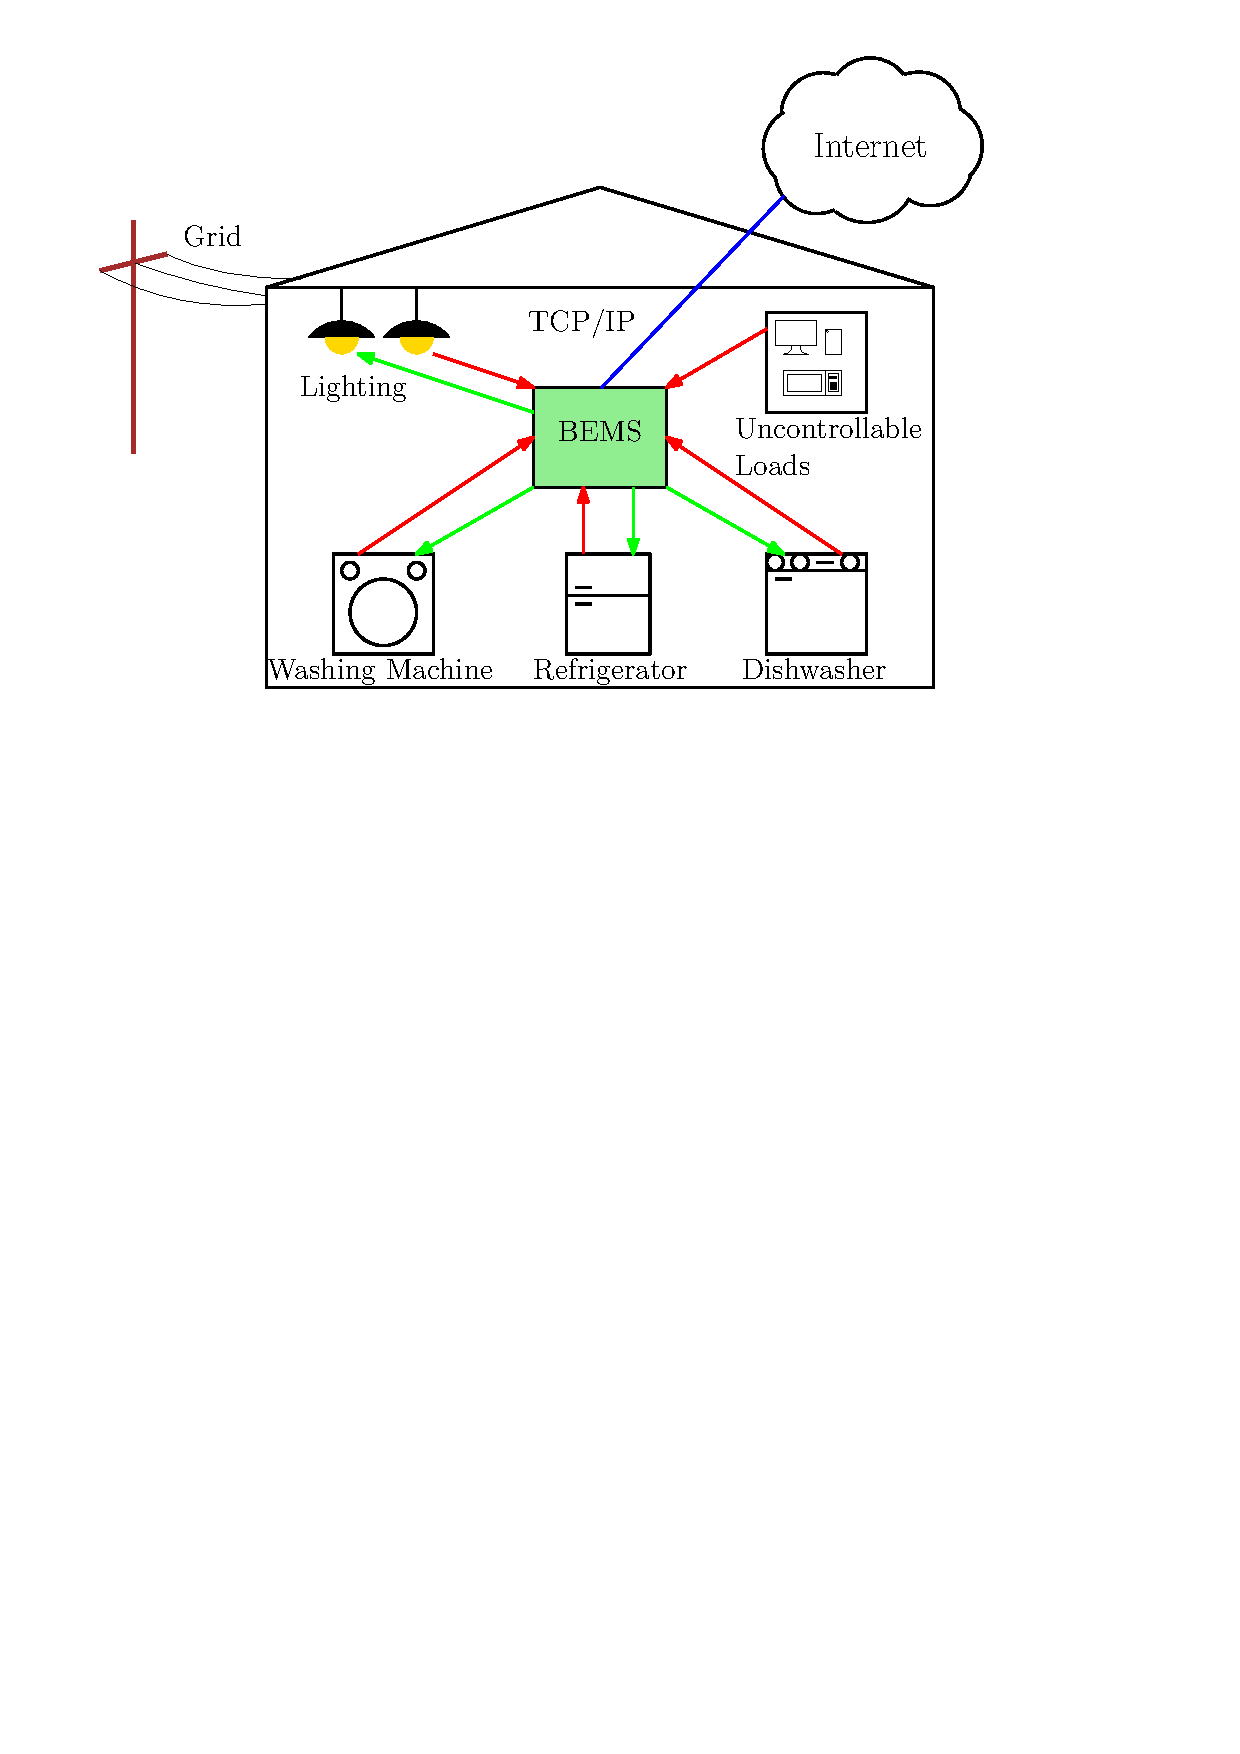
\includegraphics[scale=0.5]{figs/ipe/bemsdiagram}
  \end{figure}
\end{frame}

\begin{frame}{Introduction}{}
	\begin{figure}
		\centering
		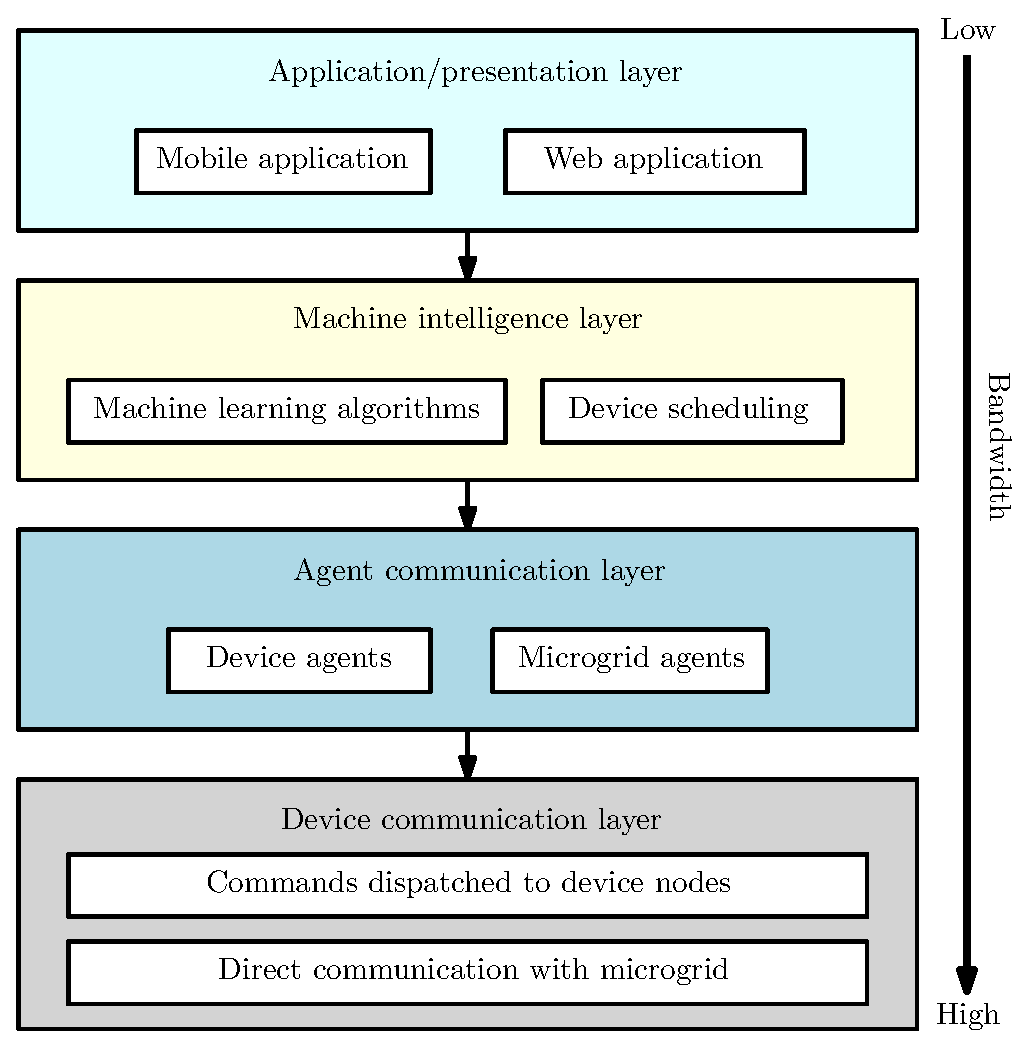
\includegraphics[scale=0.4]{figs/ipe/BEMS-softwareArchitecture}
	\end{figure}
\end{frame}

\section{Progress}
\begin{frame}{Progress}{}
\begin{itemize}
\item Built support for Insight Switch discovery and toggling on and off
\item Redesigned the web UI of the web platform
\item Based the UI off of the monitoring system at~\cite{sems}
\item Began implementing the device discovery and recognition feature
\end{itemize}
\end{frame}

\section{Demo}
\begin{frame}{Demo}{}
\center
\Huge Demonstration of WeMo API and Web UI
\end{frame}


\section{Plans}
\begin{frame}{Plans}{}
\begin{itemize}
\item Finish implementing the device discovery feature
\item Begin work on the Microgrid application and simulation
\end{itemize}
\end{frame}


% All of the following is optional and typically not needed. 
\appendix
\section<presentation>*{\appendixname}
\subsection<presentation>*{References}

\begin{frame}[allowframebreaks]
  \frametitle<presentation>{References}
    
  \begin{thebibliography}{10}
    
  \setbeamertemplate{bibliography item}[online]
  
  \bibitem{sems}
  Smart Energy Monitoring System
  \newblock \url{https://github.com/paulsayan/smart-energy-monitoring-system}
  \end{thebibliography}
\end{frame}

\begin{frame}
\center
\Huge 
Any questions?
\end{frame}
\end{document}



%%% Local Variables:
%%% mode: latex
%%% TeX-master: t
%%% End:
